\documentclass[fontsize=12pt,paper=a4,twoside]{scrartcl}
\usepackage{longtable} 
\usepackage{graphicx}
% SWP-Präambel
% C 2003-2017 Sebastian Offermann, Rainer Koschke, Karsten Hölscher
% In Zeilen 40 und 41 sind jeweils die aktuellen Daten einzutragen

\usepackage[utf8]{inputenc}     % Kodierung der Tex-Datei
\usepackage[T1]{fontenc}        % Korrekte Ausgabe von Sonderzeichen (Umlaute)
\usepackage[ngerman]{babel}     % Deutsche Einstellungen [ab \begin{document}]

\usepackage{bibgerm}            % Bibliographie
\usepackage{fancyhdr}           % obere Seitenränder gestalten
\usepackage{float}              % Floats Objekte mit [H] festsetzen
\usepackage{graphicx}           % Graphiken als jpg, png etc. einbinden
\usepackage{moreverb}           % zusätzliche verbatim-Umgebungen
\usepackage{pdflscape}          % PDF-Support für landscape
\usepackage[final]{pdfpages}    % Externe PDFs einbinden
\usepackage{stmaryrd}           % zusätzliche Symbole
\usepackage{supertabular}       % Tabellen über Seitenränder hinaus
\usepackage{tabularx}           % Tabellen mit vorgegebener Breite
\usepackage{url}                % setzt URLs schön mit \url{http://bla.laber.com/~mypage}

%%% Die Reihenfolge der folgenden Pakete muss beibehalten werden:
%%% varioref, hyperref, cleveref, bookmark
% Verweise innerhalb des Dokuments schick mit " ... auf Seite ... "
% automatisch versehen. Dazu \vref{labelname} benutzen
\usepackage[ngerman]{varioref}  % [vor hyperref für korrekte Verweise]
\usepackage[colorlinks=true, pdfstartview=FitV, linkcolor=blue,
            citecolor=blue, urlcolor=blue, hyperfigures=true,
            pdftex=true]{hyperref} % [vor bookmark wegen der Optionen]
\usepackage[ngerman]{cleveref}
\usepackage{bookmark}

\hyphenation{Arbeits-paket}     % Trennungsregeln

%%% Definitionen
\newcommand{\grad}{\ensuremath{^{\circ}} }
\renewcommand{\strut}{\vrule width 0pt height5mm depth2mm}
\newcommand{\gq}[1]{\glqq{}#1\grqq{}}

%%% Semesterkonstanten
\newboolean{langversion} %Deklaration
\setboolean{langversion}{true} %Zuweisung ist 'false' für Blockkurs
\newcommand{\jahr}[1]{2020} %2017/2018

% erstes Argument: SWP-2, zweites SWP-1
\newcommand{\highlight}[1]{\textcolor{blue}{\textbf{#1}}}
\newcommand{\variante}[2]{\ifthenelse{\boolean{langversion}}{#1}{#2}}
\newcommand{\nurlangversion}[0]%
    {\variante{\highlight{}}%Muss in SWP-2 ausgefüllt werden}}%
              {\highlight{Entfällt in SWP-1}}}
\newcommand{\swp}[0]{Software-Projekt \variante{2}{1}}
\newcommand{\semester}[0]{SoSe \jahr}

%%% Formatierungsanpassungen
% Damit Latex nicht zu lange Zeilen produziert:
\sloppy
%Uneinheitlicher unterer Seitenrand:
%\raggedbottom

% Kein Erstzeileneinzug beim Absatzanfang
% Sieht aber nur gut aus, wenn man zwischen Absätzen viel Platz einbaut
\setlength{\parindent}{0ex}

% Abstand zwischen zwei Absätzen
\setlength{\parskip}{1ex}

% Seitenränder für Korrekturen verändern
\addtolength{\evensidemargin}{-1cm}
\addtolength{\oddsidemargin}{1cm}

\bibliographystyle{gerapali}

% 1. Parameter: Euer/Eure TutorIn, z. B. {Kim Harrison}
% 2. Parameter: Abgabedatum, z. B. {05. April 2063}
% 3. Parameter: Versionsnummer, z. B. {1.1}
% 4.-9. Parameter: jeweils Name und (Uni-)Email-Adresse jedes 
%                 Gruppenmitglieds; mit einem & getrennt, z. B.
% {Robin Cowl & roco@tzi.de}
% Besteht die Gruppe aus weniger als 6 Personen, so werden die 
% übrigen Parameter leer gelassen: {}
\newcommand \swpdocument[9] {
% Lustige Header auf den Seiten
  \pagestyle{fancy}
  \setlength{\headheight}{70.55003pt}
  \fancyhead{}
  \fancyhead[LO,RE]{\swp{}\\%
                    \semester{}\\%
                    \documentTitle}
  \fancyhead[LE,RO]{Seite \thepage\\%
                    \slshape \leftmark\\%
                    \slshape \rightmark}

% Lustige Header nur auf dieser Seite (Titelseite)
  \thispagestyle{fancy}
  \fancyhead[LO,RE]{ }
  \fancyhead[LE,RO]{Universität Bremen\\%
                    FB 3 -- Informatik\\%
                    Dr. Karsten Hölscher\\%
                    TutorIn: #1}
  \fancyfoot[C]{}

% Start Titelseite
  \vspace{3cm}
  \begin{minipage}[H]{\textwidth}
    \begin{center}
      \bfseries \Large \swp{} -- \semester{}\\
      \smallskip
      \small VAK 03-BA-901.02\\
      \vspace{3cm}
    \end{center}
  \end{minipage}
  \begin{minipage}[H]{\textwidth}
    \begin{center}
      \vspace{1cm}
      \bfseries \Large \documentTitle\\
      \vfill
    \end{center}
  \end{minipage}
  \vfill
  \begin{minipage}[H]{\textwidth}
    \begin{center}
      \sffamily
      \begin{tabular}{lr}
        #4 \\
        #5 \\
        #6 \\
        #7 \\
        #8 \\
        #9 \\
      \end{tabular}
      \\[22mm]
      \itshape Abgabe: #2 --- Version #3 \\ ~
    \end{center}
  \end{minipage}
% Ende Titelseite

% Start Inhaltsverzeichnis
\newpage
  \thispagestyle{fancy}
  \fancyhead{}
  \fancyhead[LO,RE]{\swp{}\\%
                    \semester{}\\%
                    \documentTitle}
  \fancyhead[LE,RO]{Seite \thepage\\%
                    \slshape \leftmark\\~}
  \fancyfoot{}
  \renewcommand{\headrulewidth}{0.4pt}
  \tableofcontents
% Ende Inhaltsverzeichnis

% Header für alle weiteren Seiten
\newpage
  \fancyhead[LE,RO]{Seite \thepage\\%
                    \slshape \leftmark\\%
                    \slshape \rightmark}

}



%
% Und jetzt geht das Dokument los....
%
\begin{document}
\newcommand\documentTitle{Architekturbeschreibung}
\swpdocument{Dr. Karsten Hölscher}{31. Mai 2020}{1.1}%
            {Clara Maria Odinius & odinius@uni-bremen.de}%
            {Habib Mergan & habib1@uni-bremen.de}%
            {Kevin Santiago Rey Rodriguez & kev\_rey@uni-bremen.de}%
            {Liam Hurwitz & hurwitz@uni-bremen.de}%
            {Mehmet Ali Baykara & baykara@uni-bremen.de}%
            {Miguel Alejandro Caceres Pedraza & mcaceres@uni-bremen.de}%

%%%%%%%%%%%%%%%%%%%%%%%%%%%%%%%%%%%%%%%%%%%%%%%%%%%%%%%%%%%%%%%%%%%%%%%%
\section*{Version und Änderungsgeschichte}

{\em Die aktuelle Versionsnummer des Dokumentes sollte eindeutig und gut zu
identifizieren sein, hier und optimalerweise auf dem Titelblatt.}

\begin{tabular}{ccl}
Version & Datum & Änderungen \\
\hline
0.1 & 22.04.2020 & Dokumentvorlage als initiale Fassung kopiert \\
0.2 & 05.05.2020 &  Anwendungsfälle hinzugefügt\\
0.3 & 09.05.2020 & Verzeichnis für Definitionen, Akronyme und Abkürzungen hinzugefügt \\
0.4 & 12.05.2020 & erste Gedanken zur Globalen Analyse  notiert\\
0.5 & 12.05.2020 & Einflussfaktoren hinzugefügt\\
0.6 & 13.05.2020 & Einflussfaktoren bearbeitet, Problemkarten hinzugefügt\\
0.7 & 14.05.2020 & Schreibstil überarbeitet\\
0.8 & 14.05.2020 & Konzeptionelle Sicht hinzugefügt\\
0.9 & 14.05.2020 & weitere Problemkarten erstellt\\
1.0 & 15.05.2020 & Problemkarten überarbeitet\\
1.1 & 16.05.2020 & Einflussfaktoren überarbeitet\\
1.2 & 16.05.2020 & Globale Analyse überarbeitet\\
1.3 & 18.05.2020 & Zweck der Architekturbeschreibung hinzugefügt\\
1.4 & 18.05.2020 & Abkürzungen Alphabetisch sortiert\\
1.5 & 20.05.2020 & Globale Analyse überarbeitet\\
1.6 & 21.05.2020 & Konzeptionelle Sicht überarbeitet\\
1.7 & 21.05.2020 & Ausführungssicht  überarbeitet\\
1.8 & 21.05.2020 & Referenzen hinzugefügt\\
1.9 & 21.05.2020 & Ausführungssicht überarbeiet\\
2.0 & 22.05.2020 & Ausführungssicht Beschreibung ergänzt\\
2.1 & 22.05.2020 & Modulsicht png dem Dokument hinzugefügt\\
2.2 & 22.05.2020 & Zustandsdiagram png dem Dokument hinzugefügt\\




\ldots
\end{tabular}


%%%%%%%%%%%%%%%%%%%%%%%%%%%%%%%%%%%%%%%%%%%%%%%%%%%%%%%%%%%%%%%%%%%%%%%%
\section{Einführung}

\subsection{Zweck}

Diese Architekturbeschreibung beschreibt die grundlegenden Strukturen unseres 
Spiels \glqq Even Geiler Than Geiler Than Faster Than Light\grqq{}. 
Zu den Lesern gehören unser Püfer und Tutor Karsten Hölscher, die 
Gruppenmitglieder und weitere Interessierte der Fachrichtung Informatik.
Der Leser soll  hiermit zum einen den Kontext der Arbeit verstehen, 
sowie den Aufbau der Anwendung, vom Groben bis ins Detail, über viele 
Abstraktionsebenen hinweg. Somit wird nicht nur die technische Realiesierung 
des Spiels erklärt, sondern auch die allgemeinen Anforderungen an das Projekt  
und in diesem Zusammenhang  getroffene Entscheidungen.
Darüber hinaus, hilft uns eine Architekturbeschreibung dabei, 
das Projekt zu planen und strukturiert durchzuführen.


\subsection{Status}
Das Dokument beschreibt unseren ersten Entwurf und wird in der Implementierung umgesetzt.
\subsection{Definitionen, Akronyme und Abkürzungen}
  \begin{longtable}{ |  l | p{12cm} |}
    \hline
    Begriff & Definition \\ \hline
Software-Architektur &Beschreibt die grundlegende Komponenten eines
Softwaresystems.\\ \hline
Architektursicht (View) &Repräsentation eines ganzen Systems
aus der Perspektive einer kohärenten Menge von
Anliegen (IEEE P1471, 2002). \\ \hline
 Anwendungsfälle & Spezifiziert eine beliebige Menge von Aktionen, die
ein System ausführen muss, damit ein Resultat stattfindet,
welches für mindestens einen Akteur von Bedeutung
ist. \\ \hline
    Framework &Programmiergerüst, welches den Rahmen der Anwendung
bildet. Es umfasst Bibliotheken und Komponenten. \\ \hline
GUI &Steht für Graphical User Interface und kennzeichnet
eine grafische Schnittstelle, über die ein Mensch mit
einer Software interagiert.\\ \hline
 
    Libgdx & ist ein Java-Framework für plattformunabhängige Spieleentwicklung. \\
    \hline
IDE & integrierte Entwicklungsumgebung - Hilft bei der Bearbeitung von Projekten
in der Softwareentwicklung. \\     \hline
Versionskontrolle  &Hochgeladenen Versionen werden festgehalten und können
wieder hergestellt werden. \\     \hline
HTTP &Steht für Hypertext Transfer Protocol, einem zustandslosen
Protokoll zum synchronen Versenden von
Informationen über Rechnernetze.\\ \hline
Interface &Schnittstelle.\\     \hline
Javadoc  &Software-Dokumentationswerkzeug für die Programmiersprache Java. \\     \hline
JavaEE &(Java Platform Enterprise Edition) Eine Spezifikation für die transaktionsbasierte 
Ausführung von in Java programmierten Anwendungen.\\    \hline
JUnit & Frameworke für Tests für die Programmiersprache Java.\\     \hline
HTTPS &Durch Verschlüsselungstechniken gesichertes HTTP. \\ \hline
Maven  &Java Programme können standardisiert und verwaltet werden.\\     \hline
 ibrary &Sammlung von verschiedensten vorgefertigten Methoden oder Klassen.\\     \hline
Multiplayer &Spielmodus, mit mehr als einem Spieler zur gleichen Zeit.\\    \hline
Singleplayer &Spielmodus, mit einem Spieler, der gegen einen computergesteuerten
Gegner spielt. \\     \hline
Paketdiagramm &Strukturdiagramm der UML, stellt die Verbindung
zwischen Paketen, Paketimports bzw. Verschmelzungen
und deren Abhängigkeiten dar. \\ \hline
Problemkarte &Beschreiben Probleme im Zusammengang der Einflussfaktoren
und stellen Lösungen bzw. entsprechende
Strategien dar. \\ \hline
Sequenzdiagramm &Strukturdiagramm der UML, stellt den Austausch
von Nachrichten zwischen Objekten mittels einer Lebenslinie
dar. \\ \hline
Klassendiagramm &Strukturdiagramm der UML, stellt die statischen
Strukturen eines Systems dar.\\ \hline
Komponentendiagramm &Strukturdiagramm der UML, stellt Komponenten
und deren Schnittstellen dar. \\ \hline
TCP &Das Transmission Control Protocol ist ein Netzwerkprotokoll, das definiert, auf welche Art und Weise
 Daten zwischen Netzwerkkomponenten ausgetauscht werden sollen. \\ \hline
UDP &Das User Datagram Protocol, kurz UDP, ist ein minimales, verbindungsloses Netzwerkprotokoll, 
das zur Transportschicht der Internetprotokollfamilie gehört.\\ \hline
  UML &Steht für Unified Modeling Language und ist eine grafische
Modellierungssprache zur Spezifikation, Visualisierung,
Konstruktion und Dokumentation von Modellen
für Softwaresysteme. \\
    \hline
   

 \end{longtable}

\subsection{Referenzen}

\begin{itemize}
	\item Architekturbeschreibung DataColorado Software-Projekt 2 WiSe 2019/20
	\item Architekturbeschreibung RainersRaiders Software–Projekt 2 WiSe 2016/17
	\item Architekturbeschreibung SuperSaiyans Software-Projekt 2 SoSe 2019
	\item Hinweise zur Abgabe der Architekturbeschreibung für Software–Projekt 2 (Stand
	03.05.2019)

	\item Kick-Off-Folien (Stand 20. April 2020)
\end{itemize}


\subsection{Übersicht über das Dokument}

%%%%%%%%%%%%%%%%%%%%%%%%%%%%%%%%%%%%%%%%%%%%%%%%%%%%%%%%%%%%%%%%%%%%%%%%
\newpage
\section{Anwendungsfälle} \label{sec:Anwendungsfälle}
\subsection{Anmeldung}
Ein User startet das Spiel. Ein Fenster, in dem sich der  User mit Password und Namen einloggen  kann, öffnet sich. Wenn er die richtige Daten einträgt. kann das Spielt  weiter geführt werden. Falls die Daten nicht richtig sind, bekommt der User  einen Hinweis darauf und wird geben es erneut zu versuchen.
\subsection{Multi-Spieler}
Wenn der User angemeldet ist, dann kann er sehen, welche der andere User ebenfalls verbunden sind und hat entweder die Möglichkeit gegen ander User zu spielen oder aber ein Spiel gegen den Computer zu starten.
\subsection{Spielt-Starten}
Im ersten Fenster des Spiels kann der Benutzer das Raumschiff, die Waffen, welche er verwenden möchte, die Besatzung und den Schwierigkeitsgrad des Spiels auswählen. Anschließend startet das Spiel.
\subsection{Spielt-Verlauft}
Zu beginn, kann der Spieler die Besatzung in den von ihm gewählten Positionen/Sektionen des Raumschiffes positionieren. Dann kann er die Sprungtaste drücken, um die Zielplaneten auszuwählen. Der Benutzer kann dies in jeder Runde wiederholen.

Wenn der Benutzer einen Zielplaneten auswählt, kann er auf Gegner treffen und nach einem Dialogfeld gegen diese antreten.

Sobald der Benutzer gewonnen hat,  kann der Gegner sein Raumschiff reparieren, seine Besatzung heilen oder einen Sprung machen.

\subsection{Kampf-Regeln}
In einem Kampf gelten folgende Regeln:
\begin{itemize}
\item Wenn ein Kampf beginnt, kann der Benutzer seine Waffen ausrichten, um auf bestimmte Sektionen des gegnerischen Raumschiffes zu zielen.
 
\item Waffen brauchen Zeit zum Laden und Schießen.

\item Damit eine Waffe das Ziel treffen kann, muss der Gegner Schilde deaktiviert haben.

\item Um die Schilde zu deaktivieren, müssen diese zuvor x mal getroffen worden sein. Je Treffer auf das Schild,  verliert es an Stärke. Sobald die Stärke des Schildes Null ist, ist es deaktiviert.

\item Waffen treffen zu bestimmten Wahrscheinlichkeiten das Ziel.

\item Damit eine Waffe verwendet werden kann, muss die Sektion, in der die Waffe steht, funktionsfähig sein, sowie sich ein Besatzungsmitglied in selbiger Sektion aufhalten muss, damit diese auch bedient werden können.

\item Jedes Mal, wenn eine Waffe ein Raumschiff trifft, verliert sie ihren Lebenspunkt.

\item Sobald eines der beiden Raumschiffe keine Lebenspunkte mehr hat, hat es verloren.
\end{itemize}
\subsection{Pausenmodus}
Während eines Kampfes kann der Benutzer das Spiel in den Pausenmodus versetzen. Dies bedeutet, dass beide Schiffe aufhören zu schießen und die Besatzung aufhört, sich zu bewegen. Wenn das Spiel fortgesetzt wird, werden die Waffen wieder aktiviert und auch die Besatzung.
\newpage
%%%%%%%%%%%%%%%%%%%%%%%%%%%%%%%%%%%%%%%%%%%%%%%%%%%%%%%%%%%%%%%%%%%%%%%%
\section{Globale Analyse} \label{sec:globale_analyse}



\subsection{Einflussfaktoren} \label{sec:einflussfaktoren}
\textbf{Legende:}
\begin{itemize}
    \item[++] Hohe Flexibilität und Veränderlichkeit
    \item[ + ] Leichte Flexibilität und Veränderlichkeit
    \item[- - ] Sehr geringe Flexibilität und Veränderlichkeit
    \item[-   ] Wenig Flexibilität und Veränderlichkeit
  \end{itemize}
  \vspace*{20mm}
  

%{\itshape Hier sind Einflussfaktoren gefragt, die sich auf die Architektur
%beziehen. Es sind ausschließlich architekturrelevante Einflussfaktoren, und 
%nicht z.\,B.\ solche, die lediglich einen Einfluss auf das Projektmanagement 
%haben. Fragt Euch also bei jedem Faktor: Beeinflusst er wirklich die 
%Architektur? Macht einen einfachen Test: Wie würde die Architektur aussehen, 
%wenn ihr den Einflussfaktor $E$ berücksichtigt? Wie würde sie aussehen, wenn Ihr
%$E$ nicht berücksichtigt? Kommt in beiden Fällen dieselbe Architektur heraus, 
%dann kann der Einflussfaktor nicht architekturrelevant sein.

%Es geht hier um Einflussfaktoren, die
%\begin{enumerate}
%  \item sich über die Zeit ändern,
%  \item viele Komponenten betreffen,
%  \item schwer zu erfüllen sind oder
%  \item mit denen man wenig Erfahrung hat.
%\end{enumerate}

%Die Flexibilität und Veränderlichkeit müssen ebenfalls charakterisiert werden. 
%\begin{enumerate}
%  \item Flexibilität: Könnt Ihr den Faktor zum jetzigen Zeitpunkt beeinflussen?
%  \item Veränderlichkeit: ändert der Faktor sich später durch äußere Einflüsse?
%\end{enumerate}

%Unter Auswirkungen sollte dann beschrieben werden, \emph{wie} der Faktor 
%\emph{was} beeinflusst. Das können sein:
%\begin{itemize}
%  \item andere Faktoren
%  \item Komponenten
%  \item Operationsmodi
%  \item Designentscheidungen (Strategien)
%\end{itemize}

%Verwendet eine eindeutige Nummerierung der Faktoren, um sie auf den 
%Problemkarten einfach referenzieren zu können.}


%%START einflussfaktoren

%\begin{table}[H]
%\centering
\begin{longtable}{|p{3cm}|p{5cm}|p{1cm}|p{5cm}|}
\hline
Einflussfaktor& \begin{tabular}[c]{@{}l@{}}Flexibilität und \\ Veränderlichkeit\end{tabular}                                                              & \begin{tabular}[c]{@{}l@{}}++/\\\\ - -\end{tabular} & Auswirkungen                                                                                                                                                                                                                              \\ \hline
\multicolumn{4}{|l|}{O1 : Organisation}                                                                                                                                                                                                                                                                                                                                                                                                                                                                                                                                                          \\ \hline
\multicolumn{4}{|l|}{O1.1 Time-To-Market}                                                                                                                                                                                                                                                                                                                                                                                                                                                                                                                                                        \\ \hline
													 \begin{tabular}[c]{@{}l@{}}Die Auslieferung\\  erfolgt am\\  02.08.2020.\end{tabular} & \begin{tabular}[c]{@{}l@{}}Keine\\ Veränderlichkeit oder \\Flexibilität, da \\ Vorgaben bestehen.\end{tabular} & \begin{tabular}[c]{@{}l@{}}- -/\\   - -\end{tabular} & \begin{tabular}[c]{@{}l@{}}Nicht alle\\  Funktionen können\\  realisiert werden \\ bzw. implementiert werden.\end{tabular}                                                                                                                                             \\ \hline
\multicolumn{4}{|l|}{O1.2 Architektur-Abgabe}                                                                                                                                                                                                                                                                                                                                                                                                                                                                                                                                                    \\ \hline
													 \begin{tabular}[c]{@{}l@{}}Die Auslieferung \\erfolgt am\\ 31.05.2020.\end{tabular}      & \begin{tabular}[c]{@{}l@{}}Keine\\ Veränderlichkeit oder \\Flexibilität, da \\ Vorgaben bestehen.\end{tabular} & \begin{tabular}[c]{@{}l@{}}- -/\\   - -\end{tabular} & \begin{tabular}[c]{@{}l@{}}Durch den\\ Zeitdruck könnte\\ die Architektur\\ mangelhaft\\ werden. Wenn wir\\ uns nicht genug\\ Zeit lassen,\\ könnten Aspekte,\\ die relevant für die\\ Architektur sind,\\ vergessen werden.\end{tabular} \\ \hline
\multicolumn{4}{|l|}{O1.3 Entwickler}                                                                                                                                                                                                                                                                                                                                                                                                                                                                                                                                                    \\ \hline
													 \begin{tabular}[c]{@{}l@{}}Die\\ Projektgruppe \\besteht aus\\ 6 Entwicklern\\\end{tabular}      & \begin{tabular}[c]{@{}l@{}}Falls ein Entwickler \\ (temporär) ausfällt kann\\ ein anderer Entwickler\\ einspringen. \\ Keine neuen Entwickler \\
können eingestellt \\ werden. Gruppenmitglieder\\ können wegfallen oder \\ austreten\end{tabular} & \begin{tabular}[c]{@{}l@{}}+/\\   - -\end{tabular} & \begin{tabular}[c]{@{}l@{}} Die Architektur kann \\wegen Zeitmangel (es \\können nicht mehr \\als die ursprünglichen\\ sechs Entwickler\\ mitarbeiten) und \\fehlenden Fähigkeiten\\ Mängel enthalten. \\ Unvollständige\\ Implementierung droht \end{tabular} \\ \hline

\multicolumn{4}{|l|}{O1.4 Fähigkeiten Entwickler}                                                                                                                                                                                                                                                                                                                                                                                                                                                                                                                                                    \\ \hline
													 \begin{tabular}[c]{@{}l@{}}Nicht alle \\ Entwickler \\ haben die gleiche \\ Programmier-\\erfahrung \end{tabular}      & \begin{tabular}[c]{@{}l@{}}Keine Flexibilität,\\ aber Veränderlichkeit,\\ da man sich\\ einarbeiten/recherchieren \\kann. \end{tabular} & \begin{tabular}[c]{@{}l@{}}- -/\\   ++\end{tabular} & \begin{tabular}[c]{@{}l@{}}Die Implementierung \\ kann Mängel enthalten. \\\end{tabular} \\ \hline

\newpage

\hline									
\multicolumn{4}{|l|}{O1.5 Teamarbeit in Corona-Zeiten}                                                                                                                                                                                                                                                                                                                                                                                                                                                                                                                                                    \\ \hline
 \begin{tabular}[c]{@{}l@{}}
Das persönliche\\ Treffen kann \\nicht stattfinden,\\ aufgrund von\\ Kontakt- \\beschränkung \end{tabular}      & \begin{tabular}[c]{@{}l@{}} Digitale Treffen über z.B.\\ Discord. Keine \\Veränderlichkeit\\ aufgrund der \\ Gesetzeslage. \end{tabular} & \begin{tabular}[c]{@{}l@{}}++/\\   - -\end{tabular} & \begin{tabular}[c]{@{}l@{}}Missverständnisse \\können öfter\\auftreten.\\Teamarbeit könnte\\erschwert werden\\ und dadurch\\die Qualität der\\der Architektur\\beeinträchtigen
\\\end{tabular} \\ \hline
%%\end{tabular}
\end{longtable}

%%%%%%
%%%%%%

%%\begin{table}[H]
%%\centering
\begin{longtable}{|p{3cm}|p{5cm}|p{1cm}|p{5cm}|}
\hline
Einflussfaktor& \begin{tabular}[c]{@{}l@{}}Flexibilität und \\ Veränderlichkeit\end{tabular}                                                              & \begin{tabular}[c]{@{}l@{}}++/\\\\ - -\end{tabular} & Auswirkungen                                                                                                                                                                                                                              \\ \hline
\multicolumn{4}{|l|}{T1: Technik}
\\ \hline
\multicolumn{4}{|l|}{T1.1: Programmiersprache}                                                                                                                                                                                                                                                                                                                                                                                                                                                                                                                                                    \\ \hline
                                                           \begin{tabular}[c]{@{}l@{}}Java 8 \\ oder höher ist \\ vorgegeben.\end{tabular}      & \begin{tabular}[c]{@{}l@{}}Die Programmier-\\sprache wird vorgegeben.\\ Wir können aber\\zwischen verschiedenen\\Versionen auswählen.\end{tabular} & \begin{tabular}[c]{@{}l@{}}- -/\\   - -\end{tabular} & \begin{tabular}[c]{@{}l@{}}Das Architektur muss\\ in Java umgesetzt \\werden.\end{tabular} \\ \hline

\multicolumn{4}{|l|}{T1.2 Betriebssystem}                                                                                                                                                                                                                                                                                                                                                                                                                                                                                                                                                    \\ \hline
                                                           \begin{tabular}[c]{@{}l@{}}Die Anwendung \\muss auf den\\gängigen\\ Betriebssystemen\\(MacOS,\\ Windows, Linux) \\ laufen. \end{tabular}      & \begin{tabular}[c]{@{}l@{}}Keine\\ Veränderlichkeit oder \\Flexibilität, da\\ Mindestanforderungen\\ bestehen. Aber wir können\\ noch weitere\\ Betriebssysteme\\ hinzufügen\end{tabular} & \begin{tabular}[c]{@{}l@{}}- -/\\   - -\end{tabular} & \begin{tabular}[c]{@{}l@{}}Bei der Implementierung \\ müssen die gängigen\\ Betriebssysteme\\ berücksichtigt werden.\\ Wenn die Anwendung\\auf mehr\\Betriebssystemen\\laufen soll, dann\\ muss mehr Zeit\\investiert werden. \end{tabular} \\ \hline

\multicolumn{4}{|l|}{T1.3 Client-Server-Architektur}                                                                                                                                                                                                                                                                                                                                                                                                                                                                                                                                                    \\ \hline
                                                           \begin{tabular}[c]{@{}l@{}}Zur\\ Implementierung\\ muss Client-\\Server-\\Architektur\\ benutzt werden. \end{tabular}      & \begin{tabular}[c]{@{}l@{}}Keine\\ Veränderlichkeit oder \\Flexibilität, da\\ Mindestanforderungen\\bestehen.\end{tabular} & \begin{tabular}[c]{@{}l@{}}- -/\\   - -\end{tabular} & \begin{tabular}[c]{@{}l@{}}Das Projekt\\ muss eine \\Client-Server-Architektur \\haben.\end{tabular} \\ \hline

\newpage

\hline	
\multicolumn{4}{|l|}{T1.4: Framework libgdx}                                                                                                                                                                                                                                                                                                                                                                                                                                                                                                                                                    \\ \hline
                                                           \begin{tabular}[c]{@{}l@{}}Als Framework \\zur Erstellung \\der Oberfläche\\ muss libgdx\\ verwendet\\ werden.\end{tabular}      & \begin{tabular}[c]{@{}l@{}}Keine\\ Veränderlichkeit oder \\Flexibilität, da Teil der\\ Mindestanforderungen.\end{tabular} & \begin{tabular}[c]{@{}l@{}}- -/\\   - -\end{tabular} & \begin{tabular}[c]{@{}l@{}}Der Client muss\\ in libgdx umgesetzt \\werden. Der Aufwand\\ steigt, weil die\\ Gruppe ein neues\\ Framework lernen müssen\\ und daher können\\Mängel in der\\ Implementierung entstehen.\end{tabular} \\ \hline

\multicolumn{4}{|l|}{T1.5: Persistenz}                                                                                                                                                                                                                                                                                                                                                                                                                                                                                                                                                    \\ \hline
                                                           \begin{tabular}[c]{@{}l@{}}Zur \\ Speicherung der \\Daten soll\\ eine \\leichtgewichtige\\ relationale\\ Datenbank\\verwendet\\ werden.\end{tabular}      & \begin{tabular}[c]{@{}l@{}}Keine Flexibilität,\\da Mindestanforderungen\\bestehen. Veränderlich,\\ da durch überlastete\\Server auf ein\\ externes Datenbank-\\managementsystem \\umgesprungen werden \\muss.\end{tabular} & \begin{tabular}[c]{@{}l@{}}- -/\\ +\end{tabular} & \begin{tabular}[c]{@{}l@{}}Die Architektur muss \\angepasst werden, sodass\\ wir eine leichtgewichtige\\ relationale Datenbank\\ verwenden können.\\Wir entscheiden\\ uns für H2\end{tabular} \\ \hline

\multicolumn{4}{|l|}{T1.6: Build System}                                                                                                                                                                                                                                                                                                                                                                                                                                                                                                                                                    \\ \hline
                                                           \begin{tabular}[c]{@{}l@{}}Um das\\ Projekt zu bauen\\ muss ein\\ Build-System \\benutzt werden.\end{tabular}      & \begin{tabular}[c]{@{}l@{}}Auswahl zwischen\\ Maven und Gradle\\ möglich. Keine\\ Veränderlichkeit\\ möglich, da \\ Mindestanforderungen\\bestehen.\end{tabular} & \begin{tabular}[c]{@{}l@{}}+/\\   - -\end{tabular} & \begin{tabular}[c]{@{}l@{}}Das Projekt muss\\ Maven oder Gradle-build\\ fähig sein.\\ Wir verwenden Gradle\end{tabular} \\ \hline


\newpage
\hline                                
\multicolumn{4}{|l|}{T1.7: Wartbarkeit}                                                                                                                                                                                                                                                                                                                                                                                                                                                                                                                                                    \\ \hline
                                                           \begin{tabular}[c]{@{}l@{}}Die Software\\ muss einfach \\zu warten sein.\end{tabular}      & \begin{tabular}[c]{@{}l@{}}Es sind keine\\ Anforderungen bezüglich\\ der Projektstruktur\\ gegeben, daher\\ können wir\\ flexibel selbst \\entscheiden wie wir \\diese implementieren .\end{tabular} & \begin{tabular}[c]{@{}l@{}}++/\\   ++\end{tabular} & \begin{tabular}[c]{@{}l@{}}Die Architektur muss \\so aufgebaut sein,\\ sodass die Software\\ leicht gewartet und \\erweitert werden kann.\end{tabular}
\\\hline
\end{longtable}
\begin{longtable}{|p{3cm}|p{5cm}|p{1cm}|p{5cm}|}
\hline
Einflussfaktor& \begin{tabular}[c]{@{}l@{}}Flexibilität und \\ Veränderlichkeit\end{tabular}                                                              & \begin{tabular}[c]{@{}l@{}}++/\\\\ - -\end{tabular} & Auswirkungen                                                                                                                                                                                                                              \\ \hline               
\multicolumn{4}{|l|}{P1: Produktfaktoren}
\\ \hline
\multicolumn{4}{|l|}{P1.1: Spiel unterbrechen und Spielstand speichern}                                                                                                                                                                                                                                                                                                                                                                                                                                                                                                                                                    \\ \hline
                                                           \begin{tabular}[c]{@{}l@{}}Die Anwendung\\ muss in der\\ Lage sein,\\ ein zuvor von\\ einem bestimmten\\ Benutzer\\ gestartetes\\ Spiel zu speichern\\ und dem Benutzer\\ die Möglichkeit\\ zu geben,\\ es zu einem\\ anderen Zeit-\\ punkt fortzu-\\setzen. \end{tabular}      & \begin{tabular}[c]{@{}l@{}}Keine Flexibilität\\ und keine\\ Veränderlichkeit, da\\ Mindestanforderungen\\bestehen.\end{tabular} & \begin{tabular}[c]{@{}l@{}} - -/\\ - -  \end{tabular} & \begin{tabular}[c]{@{}l@{}}Wir müssen eine\\ Datenbank integrieren um\\zu speichern.\end{tabular} \\ \hline
\newpage
\hline
\multicolumn{4}{|l|}{P1.2: Schwierigkeitsstufen}                                                                                                                                                                                                                                                                                                                                                                                                                                                                                                                                                    \\ \hline
                                                           \begin{tabular}[c]{@{}l@{}}Für Benutzer\\ müssen\\ mindestens zwei\\ unterschiedliche\\ Schwierig-\\keitsgrade\\ implementiert\\ werden.\end{tabular}      & \begin{tabular}[c]{@{}l@{}}Keine\\ Veränderlichkeit,da\\ Mindestanforderungen\\ bestehen.Es können\\aber mehr als\\ zwei Schwierigkeitsgrade\\ implementiert\\werden. Außer dem\\ Karsten-Modus\\ können wir den\\ Schwierigkeitsgrad der\\ anderen Stufe \\beliebig auswählen.\end{tabular} & \begin{tabular}[c]{@{}l@{}} + /\\   - -\end{tabular} & \begin{tabular}[c]{@{}l@{}}Das Spiel soll\\ in mindestens zwei\\verschiedenen Schwierigkeits-\\stufen gespielt werden\\ können. Pro weiterer\\ Spielstufe ändert sich\\ die Architektur.\end{tabular}      \\ \hline
                                                           \multicolumn{4}{|l|}{P1.3: Multiplayer}                                                                                                                                                                                                                                                                                                                                                                                                                                                                                                                                                    \\ \hline
                                                           \begin{tabular}[c]{@{}l@{}}Der Server muss\\ einen Multiplayer\\ Modus\\ ermöglichen.\end{tabular}      & \begin{tabular}[c]{@{}l@{}}Keine\\Flexibilität oder\\ Veränderlichkeit, da\\ Mindestanforderungen\\ bestehen. Wir können\\es aber ermöglichen,\\dass mehr als zwei\\ Spieler gleichzeitig\\spielen.\end{tabular} & \begin{tabular}[c]{@{}l@{}} +/\\   - -\end{tabular} & \begin{tabular}[c]{@{}l@{}}Die Anwendung\\ darf nicht von\\ gleichzeitiger \\Verwendung von\\ zwei Nutzern\\ überfordert sein.\\  Falls mehr als\\ zwei Spieler gleichzeitig\\ spielen sollen, dann\\ muss die Architektur\\angepasst werden.\end{tabular} \\ \hline
                                                                           \multicolumn{4}{|l|}{P1.4: Singleplayer}                                                                                                                                                                                                                                                                                                                                                                                                                                                                                                                                                    \\ \hline
                                                           \begin{tabular}[c]{@{}l@{}}Der Server muss\\ einen Singleplayer\\ Modus\\ ermöglichen, falls\\ keine mensch-\\lichen Spieler\\ vorhanden sind.\end{tabular}      & \begin{tabular}[c]{@{}l@{}}Keine\\Flexibilität oder\\ Veränderlichkeit, da\\ Mindestanforderungen\\ bestehen. \end{tabular} & \begin{tabular}[c]{@{}l@{}} - -/\\   - -\end{tabular} & \begin{tabular}[c]{@{}l@{}}Implementierung eines\\ computergesteuerten \\Gegners (NPC).\end{tabular} \\ \hline
                                                           
\multicolumn{4}{|l|}{P2.0: Struktur und Eingeschaften des Raumschiffs}
\\ \hline
\multicolumn{4}{|l|}{P2.1: Aufteilung in Sektionen}                                                                                                                                                                                                                                                                                                                                                                                                                                                                                                                                                    \\ \hline
                                                           \begin{tabular}[c]{@{}l@{}}Pro Sektion\\ gibt es\\ die relevanten \\Systeme:\\
Antrieb,\\ Waffen,\\ Schutzschild\\ \end{tabular}      & \begin{tabular}[c]{@{}l@{}}Keine\\ Flexibilität oder \\Veränderlichkeit, da,\\ Mindestanforderungen\\ bestehen. Wir\\ können aber noch\\ weitere Systeme\\hinzufügen\end{tabular} & \begin{tabular}[c]{@{}l@{}}- -/\\- - \end{tabular} & \begin{tabular}[c]{@{}l@{}}Die Sektionen in \\den Raumschiffen müssen\\ die relevanten Systeme,\\ Antrieb,Waffen,Schutzschild,\\beinhalten. Falls wir\\ weitere Systeme\\ hinzufügen, dann\\ändert sich die\\Architektur. \end{tabular} 
\\ \hline
\multicolumn{4}{|l|}{P2.2: Schäden der Sektionen}                                                                                                                                                                                                                                                                                                                                                                                                                                                                                                                                                    \\ \hline
                                                           \begin{tabular}[c]{@{}l@{}}Jede Sektion\\ kann beschädigt\\ werden, wodurch\\die darin\\enthaltenen\\ Systeme\\ beschädigt\\ werden. \end{tabular}      & \begin{tabular}[c]{@{}l@{}}Keine\\ Flexibilität oder \\Veränderlichkeit, da\\Mindestanforderungen\\ bestehen.\end{tabular} & \begin{tabular}[c]{@{}l@{}}- -/\\   - -\end{tabular} & \begin{tabular}[c]{@{}l@{}}Die Beschädigung der\\ Sektionen hat weitläufige\\ Auswirkungen auf viele\\ andere Komponenten.\end{tabular} 
\\ \hline
\newpage
\hline
\multicolumn{4}{|l|}{P2.3: Ressourcen des Spiels}                                                                                                                                                                                                                                                                                                                                                                                                                                                                                                                                                    \\ \hline
                                                           \begin{tabular}[c]{@{}l@{}}Ressourcen müss-\\en implementiert\\ werden, um\\ die Spiellogik\\ auszuführen,\\ zum Beispiel:\\
* Geld\\ * Energie\\ * Hüllenintegrität \end{tabular}      & \begin{tabular}[c]{@{}l@{}}Keine\\ Flexibilität und\\ keine Veränderlichkeit, da\\ Mindestanforderungen\\ bestehen.\end{tabular} & \begin{tabular}[c]{@{}l@{}}- -/\\   - -\end{tabular} & \begin{tabular}[c]{@{}l@{}}Entscheidender Einfluss\\ auf die Umsetzung\\ des Spiels\end{tabular} 
\\ \hline
\multicolumn{4}{|l|}{P2.4: Raumschiff  Eigenschaften}                                                                                                                                                                                                                                                                                                                                                                                                                                                                                                                                                    \\ \hline
                                                           \begin{tabular}[c]{@{}l@{}}Eigenschaften\\ können durch\\ Geld verbessert\\ werden. \end{tabular}      & \begin{tabular}[c]{@{}l@{}}Keine\\ Veränderlichkeit oder \\Flexibilität, da Teil der\\ Mindestanforderungen.\end{tabular} & \begin{tabular}[c]{@{}l@{}}- -/\\   - -\end{tabular} & \begin{tabular}[c]{@{}l@{}}  Hat Auswirkungen auf \\die Veränderlichkeit der \\Systeme (Waffen usw.).\end{tabular}
 \\ \hline

\multicolumn{4}{|l|}{P3.0: Besatzung}
\\ \hline
\multicolumn{4}{|l|}{P3.1: Raumschiff hat Besatzung}                                                                                                                                                                                                                                                                                                                                                                                                                                                                                                                                                    \\ \hline
                                                           \begin{tabular}[c]{@{}l@{}}Besatzungs-\\mitglied kann\\ sich in\\ Sektionen\\ aufhalten und\\ Systeme\\ beinflussen.\end{tabular}      & \begin{tabular}[c]{@{}l@{}}Keine Flexibilität\\ und keine\\ Veränderlichkeit,\\ da Mindestanforderungen\\ bestehen.\end{tabular} & \begin{tabular}[c]{@{}l@{}}- -/\\- - \end{tabular} & \begin{tabular}[c]{@{}l@{}}Hat Auswirkungen auf\\ die Umsetzung der \\Sektionen, auf die\\ Funktionsfähigkeit der darin\\ enthaltenen Systeme und\\ auf die möglichen\\ Spielzüge eines Spielers\end{tabular} 
\\ \hline
\multicolumn{4}{|l|}{P3.2: Besatzung Eigenschaften}                                                                                                                                                                                                                                                                                                                                                                                                                                                                                                                                                    \\ \hline
                                                           \begin{tabular}[c]{@{}l@{}}Die Besatzung\\ des Schiffes\\kann Systeme/\\Sektionen \\reparieren,\\kann sterben\\kann eingestellt/\\angeheuert \\werden und hat \\Fähigkeiten\end{tabular}      & \begin{tabular}[c]{@{}l@{}}Nur flexibel \\in der Art \\der Umsetzung.\\Keine\\ Veränderlichkeit,\\ da Teil der\\ Mindestanforderungen.\\ Aber wir können\\ noch weitere\\Fähigkeiten spezifizieren\end{tabular} & \begin{tabular}[c]{@{}l@{}}- -/\\   - -\end{tabular} & \begin{tabular}[c]{@{}l@{}}Hat Auswirkungen auf\\ die Aktionen die ein\\ Besatzungsmitglied\\ ausführen kann.\end{tabular} 
\\ \hline
\newpage
\hline
\multicolumn{4}{|l|}{P3.3: Besatzung Fähigkeiten}                                                                                                                                                                                                                                                                                                                                                                                                                                                                                                                                                    \\ \hline
                                                           \begin{tabular}[c]{@{}l@{}}Die Fähigkeiten\\ der Besatzung\\ können verbessert\\ werden und\\ beeinflussen\\ die Systeme des\\ Schiffes, auf\\ dem sie arbeiten. \end{tabular}      & \begin{tabular}[c]{@{}l@{}}Keine\\ Veränderlichkeit oder \\Flexibilität, da Teil der\\ Mindestanforderungen.\end{tabular} & \begin{tabular}[c]{@{}l@{}}- -/\\   - -\end{tabular} & \begin{tabular}[c]{@{}l@{}} Hat Auswirkungen auf\\ die Aktionen die ein\\ Besatzungsmitglied\\ ausführen kann.\end{tabular} 
\\ \hline
\multicolumn{4}{|l|}{P4.0: Universum}
\\ \hline
\multicolumn{4}{|l|}{P4.1: Struktur des Universums}                                                                                                                                                                                                                                                                                                                                                                                                                                                                                                                                                    \\ \hline
                                                           \begin{tabular}[c]{@{}l@{}}Das Universum\\ muss Stationen\\ und Planeten\\ haben, die\\ vom Raumschiff\\ des Spielers\\ durchquert\\ werden. \end{tabular}      & \begin{tabular}[c]{@{}l@{}}Keine\\ Veränderlichkeit oder \\Flexibilität, da Teil der\\ Mindestanforderungen.\end{tabular} & \begin{tabular}[c]{@{}l@{}}- -/\\- -\end{tabular} & \begin{tabular}[c]{@{}l@{}}Die Architektur\\ muss ermöglichen,\\ dass sich Raumschiffe\\ im Universum \\ Stationen und Planeten\\ anfliegen können.\end{tabular} 
\\ \hline
\multicolumn{4}{|l|}{P4.2: Station/Planet Eigenschaften}                                                                                                                                                                                                                                                                                                                                                                                                                                                                                                                                                    \\ \hline
                                                           \begin{tabular}[c]{@{}l@{}}Jede Station\\ oder jeder\\ Planet kann\\ Ereignisse haben,\\ die das Spiel\\ negativ oder\\ positiv beeinflu-\\ssen. Es gibt \\fünf verschieden-\\artige Ereignisse \end{tabular}      & \begin{tabular}[c]{@{}l@{}}Keine\\ Veränderlichkeit oder \\Flexibilität, da Teil der\\ Mindestanforderungen.\end{tabular} & \begin{tabular}[c]{@{}l@{}}- -/\\   - -\end{tabular} & \begin{tabular}[c]{@{}l@{}}Die Architektur muss\\ vorsehen, dass Ereignisse\\ auf Stationen und\\ Planeten Einfluss auf den\\ Spielverlauf haben\end{tabular} 
\\ \hline
\multicolumn{4}{|l|}{P4.3: Feindliche Schiffe}                                                                                                                                                                                                                                                                                                                                                                                                                                                                                                                                                    \\ \hline
                                                           \begin{tabular}[c]{@{}l@{}}Es gibt \\mindestens\\ drei verschiedene\\gegnerische \\Raumschiffe. \end{tabular}      & \begin{tabular}[c]{@{}l@{}}Keine\\ Veränderlichkeit oder \\Flexibilität, da Teil der\\ Mindestanforderungen..\end{tabular} & \begin{tabular}[c]{@{}l@{}}- -/\\   - -\end{tabular} & \begin{tabular}[c]{@{}l@{}} Die Architektur muss\\ mindestens drei verschiedene\\ Raumschiffe vorsehen\end{tabular} 
\\ \hline
\newpage
\hline

\multicolumn{4}{|l|}{P5.0: Struktur des Kampfes}
\\ \hline
\multicolumn{4}{|l|}{P5.1: Taktische Entscheidungen}                                                                                                                                                                                                                                                                                                                                                                                                                                                                                                                                                    \\ \hline
                                                           \begin{tabular}[c]{@{}l@{}}Der Kampf\\ mit einem\\ gegnerischen\\Raumschiff \\erfolgt\\ rundenbasiert. \end{tabular}      & \begin{tabular}[c]{@{}l@{}}Keine\\ Flexibilität oder \\Veränderlichkeit, \\da Mindestanforderungen\\ bestehen.\end{tabular} & \begin{tabular}[c]{@{}l@{}}- -/\\- - \end{tabular} & \begin{tabular}[c]{@{}l@{}}Die Architektur muss\\ ermöglichen, dass nur\\ rundenbasierte Kämpfe \\stattfinden.\end{tabular} 
\\ \hline
\multicolumn{4}{|l|}{P5.2: Waffenverhalten}                                                                                                                                                                                                                                                                                                                                                                                                                                                                                                                                                    \\ \hline
                                                           \begin{tabular}[c]{@{}l@{}}Es muss\\ entschieden \\werden auf \\welche Sektion\\ des Gegners \\die Waffe \\schießen soll. \end{tabular}      & \begin{tabular}[c]{@{}l@{}}Keine\\ Flexibilität oder \\Veränderlichkeit, \\da Mindestanforderungen\\ bestehen.\end{tabular} & \begin{tabular}[c]{@{}l@{}}- -/\\   - -\end{tabular} & \begin{tabular}[c]{@{}l@{}}Die Architektur muss\\ermöglichen, dass \\entschieden werden kann\\ auf welche Sektionen \\die Waffen schießen.\end{tabular} 
\\ \hline
\multicolumn{4}{|l|}{P5.3: Verteilen von Besatzungsmitgliedern}                                                                                                                                                                                                                                                                                                                                                                                                                                                                                                                                                    \\ \hline
                                                           \begin{tabular}[c]{@{}l@{}}Während eines\\ Kampfes kann\\ die Position der\\ Besatzung auf\\ dem Schiff\\ verändert werden.\\ Der Sektions-\\wechsel wird\\ einige Zeit\\(Runden)\\ in Anspruch\\ nehmen.\\ \end{tabular}      & \begin{tabular}[c]{@{}l@{}}Nur flexibel \\in der Art \\der Umsetzung.\\Keine\\ Veränderlichkeit, da\\ Mindestanforderungen\\ bestehen.Wir können aber\\ weitere Regeln\\aufstellen für die\\Verteilung.\end{tabular} & \begin{tabular}[c]{@{}l@{}}- -/\\   - -\end{tabular} & \begin{tabular}[c]{@{}l@{}}Hat Auswirkungen auf\\ die Umsetzung der \\Sektionen, auf die\\ Funktionsfähigkeit der darin\\ enthaltenen Systeme und\\ auf die möglichen\\ Spielzüge eines Spielers\end{tabular} 
\\ \hline

\end{longtable}

\newpage
\subsection{Probleme und Strategien} \label{sec:strategien}

\begin{longtable}{|p{15cm}|}
\hline
Problem 1: Gruppenmitglieder fallen weg                                                                          
\\ \hline                                                                                                                                                                                                                                                                                                                                                                                                                                                                                                                                                        
\textbf{Beschreibung:} \\
Während des Projekts kann es dazu kommen, dass Gruppenmitglieder die Gruppe verlassen müssen oder eigenständig verlassen oder
das Gruppenmitglieder temporär ausfallen.
Das würde dazu führen, dass der Umfang des Projekts/Mindestanforderungen angepasst werden würden.
\\ \hline
\textbf{Einflussfaktoren:} \\
O1.1: Time-To-Market \\
O1.2: Architektur-Abgabe \\
O1.3: Entwickler
\\ \hline
\textbf{Strategien:} \\
S-1: Modularisierung \\
S-2: Pair-Programming
 \\ \hline
 \textbf{Entscheidung:} S-1
\\ \hline
\end{longtable}

\begin{longtable}{|p{15cm}|}
\hline
Problem 2: Zeitliche Unterschätzung des Aufwands                                                                           
\\ \hline                                                                                                                                                                                                                                                                                                                                                                                                                                                                                                                                                        
\textbf{Beschreibung:} \\
Aufgrund von fehlender Erfahrung kann es dazu kommen, dass wir die Aufgaben und deren zeitlichen Aufwand unterschätzen.
Das kann dazu führen, dass wir die Abgabetermine nicht einhalten können.
\\ \hline
\textbf{Einflussfaktoren:} \\
O1.1: Time-To-Market \\
O1.2: Architektur-Abgabe \\
O1.4: Fähigkeiten Entwickler
\\ \hline
\textbf{Strategien:} \\
S-1: Kein Fokus auf Mindestanforderungen. Features und Mindestanforderungen zeitgleich implementieren  \\
S-2: Fokus auf Mindestanforderungen und falls Zeit übrig bleibt, dann erst Features bearbeiten
 \\ \hline
 \textbf{Entscheidung:} S-2
\\ \hline
\end{longtable}
\newpage
\begin{longtable}{|p{15cm}|}
\hline
Problem 3: Covid-19                                                                           
\\ \hline                                                                                                                                                                                                                                                                                                                                                                                                                                                                                                                                                        
\textbf{Beschreibung:} \\
In Zeiten der Corona-Krise können keine persönlichen Treffen stattfinden, aufgrund des Kontaktverbots
und somit entfallen Teambuildung-Events und persönliche Treffen mit dem Tutor/Kunden.
\\ \hline
\textbf{Einflussfaktoren:} \\
O1.5: Teamarbeit in Corona-Zeiten
\\ \hline
\textbf{Strategien:} \\
S-1: Modularisierung \\
S-2: Client-Server-Architektur
 \\ \hline
 \textbf{Entscheidung:} S-1 und S-2
\\ \hline
\end{longtable}

\begin{longtable}{|p{15cm}|}
\hline
Problem 4: Missverständnisse bei Mindestanforderungen                                                                           
\\ \hline                                                                                                                                                                                                                                                                                                                                                                                                                                                                                                                                                        
\textbf{Beschreibung:} \\
Die Gruppe entwickelt eine falsche Anforderung, aufgrund von Missverständnissen.
\\ \hline
\textbf{Einflussfaktoren:} \\
O1.1: Time-To-Market \\
P1: Produktfaktoren
\\ \hline
\textbf{Strategien:} \\
S-1: Evolutionäre Prototypen entwickeln \\
S-2: Inkrementelle Auslieferungen des Produkts \\
S-3: Verschiedene Akzeptanztests durchführen
 \\ \hline
 \textbf{Entscheidung:} S-1
\\ \hline
\end{longtable}

\begin{longtable}{|p{15cm}|}
\hline
Problem 5: Fehlende Erfahrung mit den Technologien                                                                           
\\ \hline                                                                                                                                                                                                                                                                                                                                                                                                                                                                                                                                                        
\textbf{Beschreibung:} \\
Es kann sein, dass ein Teil oder die ganze Gruppe keine Erfahrungen in der Arbeit mit den vorgegebenen Technologien besitzen
und somit in Verzug kommen mit den Abgabeterminen. Das kann zu mangelhaften Implementierungen führen. 
\\ \hline
\textbf{Einflussfaktoren:} \\
O1.1: Time-To-Market \\
O1.4: Fähigkeiten Entwickler \\
T1: Technik
\\ \hline
\textbf{Strategien:} \\
S-1: Modularisierung. Einzelne Gruppenmitglieder fokussieren sich auf einzelne Technologien und schaffen sich Expertise und geben das Wissen weiter an andere Gruppenmitglieder\\
S-2: Vorzeitiges finales Festlegen auf bestimmte Technologien um Änderungen der Architektur zu einem späteren Zeitpunkt zu vermeiden \\
S-3: Entwicklung mit Technologien mit denen man schon Erfahrungen hat
 \\ \hline
 \textbf{Entscheidung:} S-1
\\ \hline
\end{longtable}

\begin{longtable}{|p{15cm}|}
\hline
Problem 6: Persistenz der Daten                                                                           
\\ \hline                                                                                                                                                                                                                                                                                                                                                                                                                                                                                                                                                        
\textbf{Beschreibung:} \\
Es muss eine Persistenz der Daten gewährleistet werden, damit Daten nicht verloren gehen bei beispielsweise Serverneustart und Spieler können ihre Spiele fortsetzen.
\\ \hline
\textbf{Einflussfaktoren:} \\
T1.5: Persistenz \\
P1.1: Spiel unterbrechen und Spielstand speichern
\\ \hline
\textbf{Strategien:} \\
S-1: Aufbau einer Datenbankverbindung für Schreib-/Lese-Aktionen und danach Schließung der Datenbankverbindung\\
S-2: Datenbankzugriffe gekapselt in der Komponente Persistence\\
S-3: Externes Datenbankmanagementsystem
 \\ \hline
 \textbf{Entscheidung:} S-2
\\ \hline
\end{longtable}

\begin{longtable}{|p{15cm}|}
\hline
Problem 7: Überlastung des Servers                                                                           
\\ \hline                                                                                                                                                                                                                                                                                                                                                                                                                                                                                                                                                        
\textbf{Beschreibung:} \\
Der Server muss ermöglichen, dass mindestens zwei verschiedene Spieler das Spiel gleichzeitig spielen können.
\\ \hline
\textbf{Einflussfaktoren:} \\
T1.3: Client-Server-Architektur \\
P1.3: Multiplayer
\\ \hline
\textbf{Strategien:} \\
S-1: Teilung der Anwendung in eine Client-Server-Architektur \\
S-2: Client und Server sind enthalten im selben Programm \\
S-3: Multithreaded Server implementieren
 \\ \hline
 \textbf{Entscheidung:} S-1
\\ \hline
\end{longtable}
\newpage
\begin{longtable}{|p{15cm}|}
\hline
Problem 8: Die Internet-Verbindung von einem oder beiden Spielern bricht ab im Multiplayer-Modus                                                                        
\\ \hline                                                                                                                                                                                                                                                                                                                                                                                                                                                                                                                                                        
\textbf{Beschreibung:} \\
Wenn das Spiel im Multiplayer-Modus gespielt wird und ein oder beide Spieler zeitweise keine Internet-Verbindung haben, 
dann soll es ermöglicht werden, dass die Spieler ihr Spiel fortsetzen können bei hergesteller Internet-Verbindung. 
\\ \hline
\textbf{Einflussfaktoren:} \\
T1.3: Client-Server-Architektur \\
T1.5: Persistenz \\
P1.3: Multiplayer \\
P1.1: Spiel unterbrechen und Spielstand speichern
\\ \hline
\textbf{Strategien:} \\
S-1: Spielstände werden, in vorher festgelegten Zeitabständen, gespeichert um dann, nachdem die Internet-Verbindung wieder hergestellt wurde, das Spiel fortzusetzen\\
S-2: Währendessen wird das Spiel pausiert und die Spieler kriegen darüber einen Bescheid sobald die Internet-Verbindung einseitig abbricht \\
S-3: Das Spiel wird abgebrochen und der Gegenspieler gewinnt die Partie
 \\ \hline
 \textbf{Entscheidung:} S-2
\\ \hline
\end{longtable}

\begin{longtable}{|p{15cm}|}
\hline
Problem 9: Die Internet-Verbindung bricht ab bei dem Spieler bei Einzelspieler-Modus                                                                       
\\ \hline                                                                                                                                                                                                                                                                                                                                                                                                                                                                                                                                                        
\textbf{Beschreibung:} \\
Wenn das Spiel im Einzelspieler-Modus gespielt wird und der Spieler zeitweise keine Internet-Verbindung hat, 
dann soll es ermöglicht werden, dass das Spiel fortgesetzt werden kann, wenn die Internet-Verbindung wieder hergestellt wurde.
\\ \hline
\textbf{Einflussfaktoren:} \\
T1.3: Client-Server-Architektur \\
T1.5: Persistenz \\
P1.1: Spiel unterbrechen und Spielstand speichern
\\ \hline
\textbf{Strategien:} \\
S-1: Spielstände werden, in vorher festgelegten Zeitabständen, gespeichert um dann, nachdem die Internet-Verbindung wieder hergestellt wurde, das Spiel fortzusetzen\\
S-2: Das Spiel wird pausiert bis die Internet-Verbindung wieder hergestellt wurde \\
S-3: Das Spiel wird abgebrochen und der Gegenspieler gewinnt die Partie
 \\ \hline
 \textbf{Entscheidung:} S-2
\\ \hline
\end{longtable}
\newpage
\begin{longtable}{|p{15cm}|}
\hline
Problem 10: Komplexität der Implementierung                                                                       
\\ \hline                                                                                                                                                                                                                                                                                                                                                                                                                                                                                                                                                        
\textbf{Beschreibung:} \\
Die Komplexität des Software und die Projektstruktur kann schnell unübersichtlich werden, wegen der Relationen zwischen den unterschiedlichen Objekten der Implementierung.
\\ \hline
\textbf{Einflussfaktoren:} \\
T1.7: Wartbarkeit
\\ \hline
\textbf{Strategien:} \\
S-1: Modulariserung der Software \\
S-2: S.O.L.I.D, Prinzipien des OOP Designs
 \\ \hline
 \textbf{Entscheidung:} S-1
\\ \hline
\end{longtable}

\begin{longtable}{|p{15cm}|}
\hline
Problem 11: Spielstände                                                                     
\\ \hline                                                                                                                                                                                                                                                                                                                                                                                                                                                                                                                                                        
\textbf{Beschreibung:} \\
Die Spielstände müssen den jeweiligen Spielern zugeordnet werden. Spieler A kann das Spiel von Spieler B (weiter-)spielen.
\\ \hline
\textbf{Einflussfaktoren:} \\
T1.3: Client-Server-Architektur\\
T1.5: Persistenz \\
P1.1: Spiel unterbrechen und Spielstand speichern
\\ \hline
\textbf{Strategien:} \\
S-1: Jeder Spieler kann eigenen Account mit Passwort erstellen und die Spiele, die dieser Spieler gestartet hat, werden diesem Spiel zugeordnet \\
S-2: Die Spielstände lokal speichern \\
S-3: Den Spielstand als beispielsweise CSV-Datei abspeichern und exportieren und bei Fortsetzung des Spiels wieder importieren und weiter spielen
 \\ \hline
 \textbf{Entscheidung:} S-1
\\ \hline
\end{longtable}

\begin{longtable}{|p{15cm}|}
\hline
Problem 12: Der Spieler kennt den Spielverlauf und die Spielregeln nicht                                                                     
\\ \hline                                                                                                                                                                                                                                                                                                                                                                                                                                                                                                                                                        
\textbf{Beschreibung:} \\
Der Spieler spielt das Spiel zum ersten Mal und ist mit der Benutzeroberfläche überfordert und möchte möglicherweise erst die Spielregeln kennen bevor das Spiel gestartet wird.
\\ \hline
\textbf{Einflussfaktoren:} \\
P1: Produktfaktoren
\\ \hline
\textbf{Strategien:} \\
S-1: (Video-)Tutorial mit Stimme/Untertitel im Menü \\
S-2: Anleitung während des Spiels mit Quick-Instructions
 \\ \hline
 \textbf{Entscheidung:} S-1
\\ \hline
\end{longtable}

%%%%%%%%%%%%%%%%%%%%%%%%%%%%%%%%%%%%%%%%%%%%%%%%%%%%%%%%%%%%%%%%%%%%%%%%
\section{Konzeptionelle Sicht} \label{sec:konzeptionell}

\begin{figure}[!ht]
	\centering
  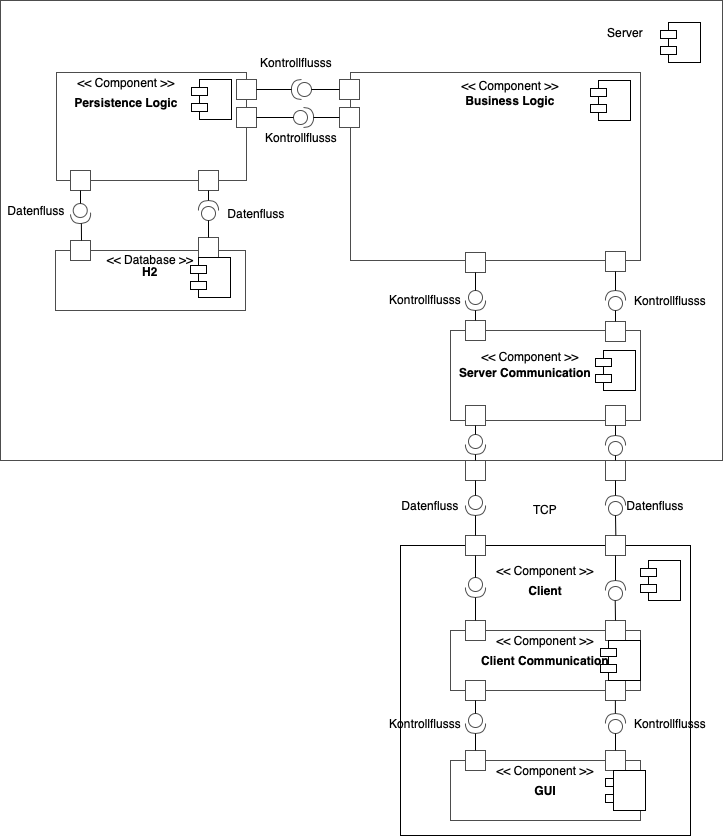
\includegraphics[width=0.85\textwidth]{Konzeptionelle_Sicht.png}
	\caption{Konzeptionelle Sicht}
	\label{fig1}
\end{figure}

In diesem Kapitel verwenden wir die konzeptionelle Sicht nach Hofmeister et al. um das System auf einer hohen Abstraktionsebene zu beschreiben.
Das Computerspiel $ " $Even Geiler Than Geiler Than Faster Than Light$ "$ wird durch eine Client-Server-Architektur realisiert.

\textbf{H2:} Die leichtgewichtige relationale Datenbank wird genutzt für die Speicherung von Daten und zum Persistieren unseres Moduls. Die Datenbank kommuniziert über JPA/Hibernate.

\textbf{DAO:TODO!}

\textbf{Business Logic:} Die Business Logic Komponente beinhaltet die Funktionalität des Systems. In unserem Fall prüft sie die von den Clients übermittelten Aktionen auf Einhaltung der Regeln und Plausibilität.
Sie nutzt die Schnittstellen Service, Model und Server Communication.
Über die Schnittstelle zu Service kann diese Komponente schreibende und lesende Zugriffe ausführen. Hierbei haben wir die Strategie der Modularisierung umgesetzt (P1 Strategie 1).

\textbf{Model:TODO!}

\textbf{Service:} Über diese Komponente werden lesende und schreibende Zugriffe auf persistente Daten in der Datenbank durchgeführt. Sie kapselt die Funktionen, die benötigt werden um auf diese Daten zuzugreifen, sodass dann nur diese Komponente lesende und schreibende Aktionen durchführen kann. Auch hierbei haben wir die Strategie der Modularisierung umgesetzt (P1 Strategie 1).

\textbf{Server Communication:} Der externe Server kommuniziert mit dem Client über eine bidirektionale TCP-Verbindung. Hierbei haben wir die Strategie der Client-Server-Architektur umgesetzt (P7 Strategie 1). Des Weiteren übermittelt diese Komponente Aktionen vom Client an die Business Logic Komponente um dort diese auf Regeln und Plausibilität zu untersuchen.

\textbf{Client Communication:} Diese Komponente stellt die Kommunikation zwischen des Clients und dem Server sicher und übermittelt Aktionen die von der GUI kommen an den Server und umgekehrt (P7 Strategie 1).

\textbf{GUI:}


%%%%%%%%%%%%%%%%%%%%%%%%%%%%%%%%%%%%%%%%%%%%%%%%%%%%%%%%%%%%%%%%%%%%%%%%
\section{Modulsicht} \label{sec:modulsicht}

{\itshape Diese Sicht beschreibt den statischen Aufbau des Systems mit Hilfe von
Modulen, Subsystemen, Schichten und Schnittstellen. Diese Sicht ist 
hierarchisch, d.\,h. Module werden in Teilmodule zerlegt. Die Zerlegung endet 
bei Modulen, die ein klar umrissenes Arbeitspaket für eine Person darstellen und
in einer Kalenderwoche implementiert werden können. Die Modulbeschreibung der 
Blätter dieser Hierarchie muss genau genug und ausreichend sein, um das Modul 
implementieren zu können.

Die Modulsicht wird durch {UML}-Paket- und Klassendiagramme visualisiert.

Die Module werden durch ihre Schnittstellen beschrieben.
Die Schnittstelle eines Moduls $M$ ist die Menge aller Annahmen, die andere 
Module über $M$ machen dürfen, bzw.\ jene Annahmen, die $M$ über seine 
verwendeten Module macht (bzw. seine Umgebung, wozu auch Speicher, Laufzeit 
etc.\ gehören).
Konkrete Implementierungen dieser Schnittstellen sind das Geheimnis des Moduls
und können vom Programmierer festgelegt werden. Sie sollen hier dementsprechend 
nicht beschrieben werden. 

Die Diagramme der Modulsicht sollten die zur Schnittstelle gehörenden Methoden
enthalten. Die Beschreibung der einzelnen Methoden (im Sinne der 
Schnittstellenbeschreibung) geschieht allerdings per Javadoc im zugehörigen 
Quelltext. Das bedeutet, dass Ihr für alle Eure Module Klassen, Interfaces und 
Pakete erstellt und sie mit den Methoden der Schnittstellen verseht. Natürlich 
noch ohne Methodenrümpfe bzw.\ mit minimalen Rümpfen. Dieses Vorgehen 
vereinfacht den Schnittstellenentwurf und stellt Konsistenz sicher.

Jeder Schnittstelle liegt ein Protokoll zugrunde. Das Protokoll beschreibt die 
Vor- und Nachbedingungen der Schnittstellenelemente. Dazu gehören die erlaubten
Reihenfolgen, in denen Methoden der Schnittstelle aufgerufen werden dürfen, 
sowie Annahmen über Eingabeparameter und Zusicherungen über Ausgabeparameter. 
Das Protokoll von Modulen wird in der Modulsicht beschrieben.
Dort, wo es sinnvoll ist, sollte es mit Hilfe von Zustands- oder 
Sequenz-diagrammen spezifiziert werden. Diese sind dann einzusetzen, wenn der
Text allein kein ausreichendes Verständnis vermittelt (insbesondere bei 
komplexen oder nicht offensichtlichen Zusammenhängen).

Der Bezug zur konzeptionellen Sicht muss klar ersichtlich sein. Im Zweifel 
sollte er explizit erklärt werden. Auch für diese Sicht muss die Entstehung 
anhand der Strategien erläutert werden.}


%%%%%%%%%%%%%%%%%%%%%%%%%%%%%%%%%%%%%%%%%%%%%%%%%%%%%%%%%%%%%%%%%%%%%%%%
\section{Datensicht} \label{sec:datensicht}

{\itshape Hier wird das der Anwendung zugrundeliegende Datenmodell beschrieben. 
Hierzu werden neben einem erläuternden Text auch ein oder mehrere 
{UML}-Klassendiagramme verwendet. Das hier beschriebene Datenmodell wird u.\,a.\ 
jenes der Anforderungsspezifikation enthalten, allerdings mit 
implementierungsspezifischen Änderungen und Erweiterungen. Siehe die gesonderten
Hinweise.}


%%%%%%%%%%%%%%%%%%%%%%%%%%%%%%%%%%%%%%%%%%%%%%%%%%%%%%%%%%%%%%%%%%%%%%%%
\section{Ausführungssicht} \label{sec:ausfuehrung}



In diesem Absatz wird die Ausführungssicht des Systems beschrieben. Diese enthält die Kommunikation bzw. die Interaktion der Komponenten und auch deren Hostrechner, auf denen die Komponenten laufen. \\Die untenstehende Abbildung dient als Ausführungssicht für das Spiel $ " $Even Geiler Than Geiler Than Faster Than Light$ "$ . Das Spiel wird mit dem Client-Server Architektur Pattern realisiert.\\
\begin{figure}[htp]
	\centering
	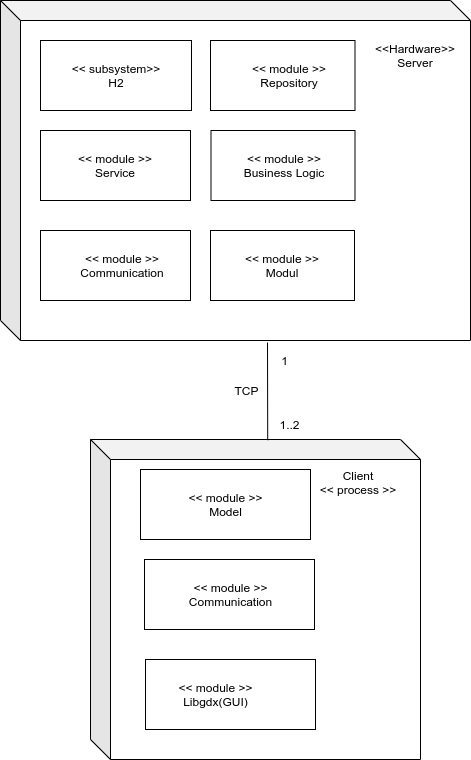
\includegraphics[width=0.5\linewidth]{Ausfuehrungsicht_Diagram.png}
	\caption{Ausführungssicht}
	\label{fig2}
	
\end{figure}
\newpage
Die Abbildung besteht aus zwei geteilten Boxen. Der oberste Teil repräsentiert den Server und enthält mehrere Module sowie Service, Datenbank(H2), Business Logic, Communication und DAO(Data Access Object). Der Server kommuniziert durch TCP mit dem Client. Es können ein bis zwei Clients bzw. Spieler gleichzeitig mit dem Server kommunizieren. Der Server stellt die Verbindung mit der Datenbank sicher, indem er über das Service-Modul interagiert. Dadurch, dass wir Daten speichern müssen benötigen wir eine Datenbank. Mit Hilfe des DAO-Moduls werden die Daten persistiert und verwaltet. Die ausgewählte leichtgewichtige Datenbank(H2) wird mit dem Anwendungsserver auf dem selben Gerät laufen. 
\\
Der untere Teil repräsentiert den Client und besteht aus drei Modulen wie Model, Communication und GUI. Der Client wird durch TCP den Server ansprechen. Der Client interagiert mit der GUI, diese Eingaben werden dann über die Client Communication weiter an die Server Communication.


%%%%%%%%%%%%%%%%%%%%%%%%%%%%%%%%%%%%%%%%%%%%%%%%%%%%%%%%%%%%%%%%%%%%%%%%
\section{Zusammenhänge zwischen Anwendungsfällen und Architektur}
\sectionmark{Zusammenhänge AF u. Architektur} \label{sec:anwendungsfaelle}

{\itshape In diesem Abschnitt sollen Sequenzdiagramme mit Beschreibung(!) für 
\variante{zwei bis drei von Euch ausgewählte Anwendungsfälle}%
{einen von Euch ausgewählten Anwendungsfall}
erstellt werden. Ein Sequenzdiagramm beschreibt den Nachrichtenverkehr zwischen 
allen Modulen, die an der Realisierung des Anwendungsfalles beteiligt sind. 
\variante{Wählt die Anwendungsfälle so, dass nach Möglichkeit alle Module Eures
entworfenen Systems in mindestens einem Sequenzdiagramm vorkommen. Falls Euch 
das nicht gelingt, versucht möglichst viele und die wichtigsten Module 
abzudecken.}%
{Dazu könnt ihr Euch einen Anwendungsfall heraussuchen, der möglichst viele 
Module der  Architektur abdeckt. In SWP-2 werden wir mehrere Anwendungsfälle
betrachten und eine umfangreichere Abdeckung der Architektur anstreben.} }

\textbf{1. New Game}\\
\textbf{2. Spiel unterbrechen und fortsetzen}\\
\textbf{3. Waffensystem kaufen}
%%%%%%%%%%%%%%%%%%%%%%%%%%%%%%%%%%%%%%%%%%%%%%%%%%%%%%%%%%%%%%%%%%%%%%%%
\section{Evolution} \label{sec:evolution}

{\itshape Beschreibt in diesem Abschnitt, welche Änderungen Ihr vornehmen müsst,
wenn sich Anforderungen oder Rahmenbedingungen ändern. Insbesondere würden 
hierbei die in der Anforderungsspezifikation unter \glqq{}Ausblick\grqq{} 
genannten Punkte behandelt werden.}

\dots

\end{document}

%%% Local Variables: 
%%% mode: latex
%%% mode: reftex
%%% mode: flyspell
%%% ispell-local-dictionary: "de_DE"
%%% TeX-master: t
%%% End: 
